\part{解析几何}
所谓解析几何，可以称之为懒人的几何

所谓解析几何，可以称之为懒人的几何

所谓解析几何，可以称之为懒人的几何

所谓解析几何，可以称之为懒人的几何

所谓解析几何，可以称之为懒人的几何

所谓解析几何，可以称之为懒人的几何

所谓解析几何，可以称之为懒人的几何

所谓解析几何，可以称之为懒人的几何

所谓解析几何，可以称之为懒人的几何

所谓解析几何，可以称之为懒人的几何

所谓解析几何，可以称之为懒人的几何

所谓解析几何，可以称之为懒人的几何

所谓解析几何，可以称之为懒人的几何

所谓解析几何，可以称之为懒人的几何

所谓解析几何，可以称之为懒人的几何

所谓解析几何，可以称之为懒人的几何

所谓解析几何，可以称之为懒人的几何

所谓解析几何，可以称之为懒人的几何

所谓解析几何，可以称之为懒人的几何

所谓解析几何，可以称之为懒人的几何

所谓解析几何，可以称之为懒人的几何

所谓解析几何，可以称之为懒人的几何

所谓解析几何，可以称之为懒人的几何

所谓解析几何，可以称之为懒人的几何

所谓解析几何，可以称之为懒人的几何

所谓解析几何，可以称之为懒人的几何

所谓解析几何，可以称之为懒人的几何

所谓解析几何，可以称之为懒人的几何

所谓解析几何，可以称之为懒人的几何

所谓解析几何，可以称之为懒人的几何

所谓解析几何，可以称之为懒人的几何

所谓解析几何，可以称之为懒人的几何

所谓解析几何，可以称之为懒人的几何

所谓解析几何，可以称之为懒人的几何

所谓解析几何，可以称之为懒人的几何

所谓解析几何，可以称之为懒人的几何

所谓解析几何，可以称之为懒人的几何

所谓解析几何，可以称之为懒人的几何

所谓解析几何，可以称之为懒人的几何

所谓解析几何，可以称之为懒人的几何

所谓解析几何，可以称之为懒人的几何

所谓解析几何，可以称之为懒人的几何

所谓解析几何，可以称之为懒人的几何

所谓解析几何，可以称之为懒人的几何

所谓解析几何，可以称之为懒人的几何

所谓解析几何，可以称之为懒人的几何


我们在平面几何和立体几何里, 所用的研究方法是以公理为基础, 直接依据图形的点、线、面的关系来研究 图形的性质. 在将要学习的平面解析几何里, 所用的研究方法和平面几何、立体几何不同, 它是在坐标系的基础 上, 用坐标表示点, 用方程表示曲线 (包括直线), 通过研究方程的特征间接地来研究曲线的性质. 因此可以说, 解 析几何是用代数方法来研究几何问题的一门数学学科.
平面解析几何研究的主要问题是: (1) 根据已知条件, 求出表示平面曲线的方程; (2) 通过方程, 研究平面曲线的性质.
解析几何的这种研究方法, 在进一步学习数学、物理和其他科学技术中经常使用. 在十七世纪, 法国数学家笛卡儿创始了解析几何. 解析几何的产生对数学发展, 特别是对微积分的出现起了 促进作用; 恩格斯对笛卡儿的这一发现给予了高度的评价.
\chapter{解析几何（一）}
\section{平面解析几何简介}
\subsection{平面直角坐标系中的基本公式}
所谓解析几何，就是用坐标研究点，用方程研究曲线。在初中的时候，就已经学习过了数轴，且认定这样的事实：
实数和数轴上的点是一一对应的。那么用实数研究数轴上的点，衡量线段的长度就是自然而然的了。
\vspace*{-5pt}
\begin{figure}[h]
    \centering
    \begin{tikzpicture}
        % Draw the number line
        \draw[->] (-1,0) -- (5,0) node[right] {$x$};
    
        % Draw the points x1 and x2
        \filldraw (1,0) circle (1pt) node[below] {$x_1$} node[above]{$A$};
        \filldraw (3,0) circle (1pt) node[below] {$x_2$} node[above]{$B$};
    \end{tikzpicture}
\end{figure}
\vspace*{-5pt}
\begin{theorem}\label{数轴上的距离}在数轴上有两点\(A,B\)，坐标分别为\(x_1,x_2\)。记\(A,B\)之间的距离为\(d\)，则
    \begin{equation}
        d=|x_1-x_2|
    \end{equation}
\end{theorem}

关于\(A,B\)两点之间的距离，使用\(|AB|,|\ve{AB}|\)都是可以的；而\(AB\)这种表示既可以
表示\(A,B\)两点之间的距离，也可以表示过\(A,B\)两点的直线，使用的时候需要注意避免歧义。在写出
如\(AB\pxqdy CD\)，意味着\(|AB|=|CD|\)，且过\(AB\)两点的直线平行于过\(CD\)两点的直线。

\begin{definition}
    在定理\ref{数轴上的距离}的基础上，再加入一个点\(C\)，使得\(|AC|,|BC|\)之间总保持着一定的比例关系
，则称点\(C\)为定比分点。这个定义可以任意地推广到其他有距离的情形。若\(C\)在\(A,B\)之间，称\(C\)为内分点；
若\(C\)在\(A,B\)两侧，称\(C\)为外分点。
\end{definition}
\begin{theorem}
    在数轴上有\(A,B,C\)三点，坐标分别为\(x_1,x_2,x_3\)。若满足\(\ve{AC}=\lambda\ve{CB} \ (\lambda\neq 1)\)，
    则\begin{equation}
        x_3=\frac{x_{1}+\lambda x_{2}}{1+\lambda} \quad(\lambda \neq-1)
    \end{equation}
\end{theorem}

而在平面上也可以研究相似的问题。在下文中如果没有特殊说明，平面上的坐标总是平面直角坐标系中的坐标，
即在平面内取一组正交单位基底得到的。

\begin{theorem}[两点之间距离公式]
    在平面直角坐标系中，有\(A,B\)两点，坐标分别为\((x_1,y_1),(x_2,y_2)\)。记\(A,B\)之间的距离为\(d\)，则
    \begin{equation}
        d=\sqrt{(x_1-x_2)^2+(y_1-y_2)^2}
    \end{equation}
\end{theorem}
\begin{proof}
    
\end{proof}
\begin{exercise}
    已知三点\(A(3,2),B(0,5),C(4,6)\)，判断\(\tri ABC\)形状。
\end{exercise}



\begin{theorem}
    在数轴上有\(A,B,C\)三点，坐标分别为\((x_1,y_1),(x_2,y_2),(x_3,y_3)\)。若满足\(\ve{AC}=\lambda\ve{CB} \ (\lambda\neq 1)\)，则
    \begin{equation}
        x_3=\frac{x_{1}+\lambda x_{2}}{1+\lambda}, y_3=\frac{y_{1}+\lambda y_{2}}{1+\lambda}
    \end{equation}
\end{theorem}
\begin{corollary}\label{定比分点公式定理}
    点\(P\)为线段\(AB\)的中点，\(A,B\)坐标为$(x_1,y_1),(x_2,y_2)$，则点\(P\)坐标为
    \begin{equation}\label{定比分点公式}
        \left(\frac{x_{1}+x_{2}}{2}, \frac{y_{1}+y_{2}}{2}\right)
    \end{equation}
\end{corollary}
\begin{example}\label{三等分点}
    点\(P\)为线段\(AB\)的三等分点中更靠近\(A\)点的一个，\(A,B\)坐标为$(x_1,y_1),(x_2,y_2)$，
    求\(P\)点坐标。
\end{example}

需要使用定比分点坐标公式的时候，往往不会直接给出形如\(\ve{AC}=\lambda\ve{CB} \ (\lambda\neq 1)\)的式子。
可以根据自己的需求灵活地重新选定起点、终点和分点，
一但选定，\(\lambda\)也就随之而定。因此解题时，必须说明\(\lambda\)的意义。
在解答题中，不要直接写如式\ref{定比分点公式}，而是仿照定理\ref{定比分点公式定理}和例\ref{三等分点}推导想要的形式即可。

\begin{theorem}
    在\(\tri ABC\)中，点\(A,B,C\)的坐标分别为\((x_1,y_1),(x_2,y_2),(x_3,y_3)\)。则\(\tri ABC\)的重心
    坐标为
    \begin{equation}
        \left(\frac{x_{1}+x_{2}+x_{3}}{3},  y=\frac{y_{1}+y_{2}+y_{3}}{3} .\right)
    \end{equation}
\end{theorem}

在学习了平面直角坐标系中的基础——坐标与距离的求法之后，来了解一些简单的应用——
建立适当的坐标系解决几何问题。实际上，上面坐标与距离的知识，以及用坐标解决问题在向量
已经了解很多了，这里只是再拿出来汇总一下。
%坐标法解决问题在向量里将很多了吧，就别在这炒冷饭了，，，
\begin{example}
在$ \parallelogram A B C D $中，求证： 
\begin{equation}
    A C^{2}+B D^{2}=2\left(A B^{2}+A D^{2}\right)
\end{equation}
\end{example}
\begin{exercise}
    已知  $A B C D $ 是一个长方形, 且 $ M $ 是 $ A B C D  $所在平面上任意一个点, 求证: $ A M^{2}+C M^{2}=B M^{2}+D M^{2} $
\end{exercise}


接下来谈一谈“距离”这个词。提起距离，大家总会默认这样的事实：两点之间用线段连接起来的那段长度
才叫距离。但是在现实生活中，总是能走直线吗？在高楼林立的城市中，你必须沿着纵横的街道走（暂时忽视地球是个球这件事）；
在中国象棋的棋盘上，除了马、象，其他棋子总是只能走横纵的直线的。将这种现象抽象成数学语言，就是在平面直角坐标系中有两点\((x_1,y_1),(x_2,y_2)\)，则
\(|x_1-x_2|+|y_1-y_2|\)也一定程度上可以衡量两点之间的距离。

但是还有一个问题等待着回答：究竟什么是距离？依赖于直觉，应该可以给出这样的一些特征：
距离至少不能是负数；距离之间应该是对称的，即从\(A\)到\(B\)的距离应该等于
从\(B\)到\(A\)的距离……
\begin{definition}[距离空间]
    设$X$为非空集合，在$X$上定义一个双变量的实值函数\(\rho:X\times X\rightarrow\mathbb{R}\)，
    若对于任意的\(x,y,z\in X\)满足下列条件：
    \begin{enumerate}[(1)]
        \setlength{\itemsep}{-\itemsep}
        \item 正定性\(\rho(x,y)\leq 0,\rho(x,y)=0\Leftrightarrow x=y\)
        \item 对称性\(\rho(x,y)=\rho(y,x)\)
        \item 三角不等式\(\rho(x,y)\leq \rho(x,z)+\rho(z,y)\)
    \end{enumerate}
    则称\((X,\rho)\)为一个以\(\rho\) 为距离（或度量）的距离（度量）空间，函数\(\rho\)为其上的一个距离函数。
\end{definition}
\begin{example}求证
  \[ d_1((x_1,y_1),(x_2,y_2))=|x_1-x_2|+|y_1-y_2|\]和
    \[d_2((x_1,y_1),(x_2,y_2))=\sqrt{(x_1-x_2)^2+(y_1-y_2)^2}\]都是\(\mathbb{R}^2\)上的距离（度量）函数。
\end{example}
\begin{proof}
    正定性和对称性都是显然的，仅证明满足三角不等式即可。前者依赖于绝对值不等式，后者由几何意义即证。
    \begin{align*}
        &d_1((x_1,y_1),(x_3,y_3))+ d_1((x_2,y_2),(x_3,y_3))\\
        =&|x_1-x_3|+|y_1-y_3|+|x_3-x_2|+|y_3-y_2|\\
        \leq&|x_1-x_3+x_3-x_2|+|y_1-y_3+y_3-y_2|\\
        =&d_1((x_1,y_1),(x_2,y_2))\\
    \end{align*}
\end{proof}
实际上有这样较强的定理：
\begin{theorem}
    \((\mathbb{R}^n,\rho_p),p\leq 1\)是距离空间，其中
    \[\rho_p(x,y)=\left(\sum_{k=1}^{n}|x_k-y_k|^p\right)^{\frac{1}{p}}\]
    三角不等式由Minkowski不等式保证。
\end{theorem}

当然，这些东西的用处还太过遥远，距离是用来刻画收敛的一个强力工具，在分析学中你还会再见到它，如果不幸学了数学。

\clearpage








\subsection{曲线与方程}
在初中和高一的学习中，已经接触到了许多关于曲线与方程的知识。坐标系沟通了
代表几何的曲线与代表代数的方程。通过几何图形，可以快速认识到（或是简单地猜测）
对称性、取值范围、最值与极值等性质，同时可以反哺代数，有意识地处理一个陌生的方程。

举个具体的例子：还记得你是怎么研究一次函数\(y=2x\)的吗？或许你列了这样的一个表：
\begin{table}[h]\centering
        \begin{tabular}{|c|l|l|l|l|l|}
        \hline
        $x $   &$ -2$ & $-1$ & $0$ &$ 1$ & $2$ \\ \hline
        $y=2x$ & $-4 $&$ -2 $& $0$ & $2$ & $4$ \\ \hline
        \end{tabular}
\end{table}\\然后把它们绘制在了平面直角坐标系中，并用平滑的曲线连接起来——这里是一条直线。虽然你可能不知为什么
要这么做，但是你也大胆的猜测：如果把所有\(x\)可能的取值对应的点都绘制出来，那么一定是这条直线。
这样的研究方法在暗示着一件事：符合方程的坐标对应的点在方程对应的曲线上，完成了从代数到几何的跨越。
那你立刻就可以说出另外一个方向——从几何到代数：在曲线上的点对应的坐标符合方程。由此，抽象出下面的定义：

\begin{definition}\label{方程的曲线}
    一般地，在平面直角坐标系中，如果某曲线$C$（看作点的集合或适合某种条件的点的轨迹）上的点与一个二元
方程\[f(x,y)=0\]的实数解建立了如下的关系：
\vspace*{-8pt}
\begin{enumerate}[(1)]
    %\setlength{\itemsep}{0pt}
    \setlength{\itemsep}{-\itemsep}
    \item 曲线上点的坐标都是这个方程的解；
    \item 以这个方程的解为坐标的点都是曲线上的点．
\end{enumerate}
\vspace*{-8pt}
那么,这个方程叫做曲线的方程；这条曲线叫做方程的曲线(curve)，有时也称方程的轨迹。

此时可以将曲线$C$看做是如下的一个集合：
\vspace*{-10pt}
\[\{(x,y)\in\mathbb{R}^2|f(x,y)=0\}\]
\end{definition}
利用这个定义，可以解决下面的例题与练习。
\begin{example}判断下列说法正误，并说出理由。

    $(1)$三角形的一条中线上至少有两个点在$x$轴上，所以这条中线的方程是$y=0$。

    \((2)\)曲线\(C\)上无数个点的坐标都满足方程$F(x,y)=0$，
    方程$F(x,y)=0$的所有实数解为坐标的点都在曲线$C$
    上，所以曲线\(C\)是方程$F(x,y)=0$的曲线。
\end{example}
\begin{jie}
    两句话都不对。

    \((1)\)三角线中线是一条线段，中线上两点在\(x\)轴上，只说明中线在\(x\)轴上，或中线所在的直线是\(x\)轴，但中线不是\(x\)轴。
    换句话说，在三角形外的轴上的点，它的坐标为\((x_0,0)\)，满足方程$y=0$，但它不
    在中线上，不满足曲线与方程定义的第二个条件，所以不能说中线的方程为\(y=0\)。

    \((2)\) 曲线 $ C $ 上无数点的坐标都满足方程$  F(x, y)   =0$ , 
    不能保证曲线  $C $ 上每一个点的坐标都满足方程  $F(x ,  y)=0$ 。
    用\((1)\)的例子即可，考虑\(y=0,\ x\in(-1,1)\)作为\(F(x,y)\)，\(x\)轴作为
    曲线\(C\)。因此，不满足曲线与方程定义的第一个条件， 不能说曲线  $C$  是方程 $ F(x, y)=0$  的曲线。
\qed
\end{jie}

通过这个例子是想要说明，定义\ref{方程的曲线}并不是废话。从集合的观点，曲线可以看作是具有
某种本质特征（条件）的点的集合，或者看作是动点按照某种运动规律运动的轨迹，但是总要通过严格的定义保证：
这条曲线上的点都具有这种本质特征 \textcolor{red}{（纯粹性）}，具有这种本质特征的点都在这条曲线上 \textcolor{red}{（完备性）}。
\begin{example}
若\((x,2)\)在曲线\(x^2+xy+y^3=9\)上，求\(x\)的值。
\end{example}
\begin{jie}
    点在曲线上，故点对应的坐标是方程的解。带入其中得到
    \[x^2+2y+8=9\]

    解得\(x=-1\pm\sqrt{2}\)
    \qed
\end{jie}

\begin{example}
    求方程\((x-y)^2+(xy-1)^2=0\)表示的曲线。
\end{example}
\begin{jie}
    由于\((x-y)^2\leq 0,(xy-1)^2\leq 0\)，又\((x-y)^2+(xy-1)^2=0\)，故总有
    \((x-y)^2=0\)且\((xy-1)^2=0\)。仅有\((1,1),(-1,-1)\)符合。
    \qed
\end{jie}
\begin{exercise}
    若曲线\(ax^3+by^2=4\)经过了\((0,2)\)和\((\sqrt[3]{2},1)\)，求该曲线方程。
\end{exercise}
\begin{exercise}
    求方程\(x^2+4xy+4y^2=9\)表示的曲线。
\end{exercise}

接下来了解一下，如果根据曲线求出曲线对应的方程。

\begin{example}
    求平分一、三象限的直线方程。
\end{example}
\begin{jie}
    由角平分线的判定定理，在角的内部到角的两边距离相等的点在角平分线上。设角平分线上点为\(P(x,y)\)，故
    这些点构成的集合是\[\{P|d_{P-x\text{轴}}=d_{P-y\text{轴}}\}\]
    点\((x,y)\)到\(x\)轴
    距离为\(|y|\)，到\(y\)轴距离为\(|x|\).故
    \[|x|=|y|\]
    解出来\(x=\pm y\)，其中\(y=-x\)不在一三象限的内部，舍去。仅考虑\(y=x\)：符合方程的坐标对应的点在一、三角平分线上，
    一、三象限角平分线上的点也符合\(y=x\)。故平分一、三象限的直线方程为\(y=x\)。
    \qed
\end{jie}
\begin{comment}
解出来两条直线，一条是内角平分线，另一条是外角平分线。在这里\(y=-x\)是第二、四象限角平分线。
\end{comment}
归纳出如下步骤：
\tbox{
\begin{enumerate}[(1)]
    \setlength{\itemsep}{-\itemsep}
    \item 建立适当的坐标系，用有序实数对\((x,y)\)表示曲线上任意一点M的坐标；
    \item 写出适合条件\(p\)的点\(M\)的集合 $P=\{M|p(M)\}$；
    \item 用坐标表示条件$p(M)$，列出方程\(f(x,y)=0\)；
    \item 化方程\(f(x,y)=0\)为最简形式；
    \item 说明以化简后的方程的解为坐标的点都在曲线上，如果某个点是方程的解却不在曲线上要剔除。
\end{enumerate}
    }
\begin{example}
    已知两点 $ A(-2,-2), B(2,2)$ ，试求满足条  $||M A|-|M B||=4$  的动点  M  的轨迹方程。
\end{example}
\begin{jie}
    设动点  $M $ 的坐标为 $ (x, y)$  ，则由条件$||M A|-|M B||=4$
    可得
    
   $$ |\sqrt{(x+2)^{2}+(y+2)^{2}}-\sqrt{(x-2)^{2}+(y-2)^{2}}|=4,$$
    移项得
    
   $$ \sqrt{(x+2)^{2}+(y+2)^{2}}=\sqrt{(x-2)^{2}+(y-2)^{2}}\pm 4$$
    两边平方, 整理得
    
  $$\pm \sqrt{(x-2)^{2}+(y-2)^{2}}=x+y-2 $$
    再次平方得
   $$ x y=2$$

   其上一点\(P\)不妨表示为\((x,\dfrac{2}{x})\)，到\(A,B\)两点距离为
   \[|PA|=\sqrt{(x+2)^2+(\frac{2}{x}+2)^2}=\sqrt{(x+\frac{2}{x}+2)^2}=|x+\frac{2}{x}+2|\]
    \[|PB|=\sqrt{(x-2)^2+(\frac{2}{x}-2)^2}=\sqrt{(x+\frac{2}{x}-2)^2}=|x+\frac{2}{x}-2|\]
    由基本不等式可知，\(x+\dfrac{2}{x}\geq 2\sqrt{2}\)或\(x+\dfrac{2}{x}\leq -2\sqrt{2}\)，由此脱下绝对值，总满足
    \[||M A|-|M B||=4\]
    故以方程的解为坐标的点都满足该动点的条件，\(xy=2\)就是所求轨迹的方程。
    \qed
\end{jie}
方程化简到什么程度，并没有明确的规定，一般指
将方程\(f(x,y)=0\)化成关于\(x,y\)的整式。如果化简过程破坏了同解
性，就需要剔除不属于轨迹上的点，找回属于轨迹而遗漏的点。化简方程时候，要尽量保证方程的同解性，在平方、去绝对值、去分母的时候要尤其
谨慎。

利用下面两个练习，初步学习如何将几何条件翻译为坐标语言。
\begin{exercise}
    在平面直角坐标系中，\(A\ (-1,-1),B\ (3,7)\)，求线段\(AB\)的垂直平分线的方程。
\end{exercise}
\begin{hint}
    到线段两端距离相等的点在线段的垂直平分线上。
\end{hint}
\begin{exercise}
    在平面直角坐标系中，已知点$M(4,0),N(1,0)$，若动点P满足$\overrightarrow{MN}\cdot\overrightarrow{MP}=6|\overrightarrow{NP}|$。求
动点$P$的轨迹$C$的方程。
\end{exercise}
\begin{hint}
    向量关系可以翻译为坐标关系。
\end{hint}
\begin{exercise}
    下列方程表示同一曲线的一组是
    \begin{enumerate}[(1)]
        \setlength{\itemsep}{-\itemsep}
        \item \(xy=1\)，\(y=\dfrac{1}{x}\)
        \item \(y=|x|\)，\(y=\pm x\)
        \item \(y=\dfrac{x^2-1}{x-1}\)，\(y=x+1\)
        \item \(y=\sqrt{1-x^2}\)，\(x^2+y^2=1\)
    \end{enumerate}
\end{exercise}

接下来在认识一下，如何借助已知轨迹方程，去求其他的轨迹方程。
\begin{example}在平面直角坐标系中，\(O\)为坐标原点。已知圆$C:x^2+(y-3)^2=9$，过原点作圆$C$的弦$OP$，
求$OP$的中点$Q$的轨迹方程。
\end{example}
\begin{jie}

\end{jie}
\begin{exercise}
    动点\(P\)为曲线\(y=2x^2+1\)上任意一点，定点\(A(0,-1)\)，线段\(PA\)上有一点\(M\)，
    满足\(PM:AM=1:2\)，求\(M\)点轨迹方程。
\end{exercise}
\tbox{用相关点法求解轨迹：
\begin{enumerate}[(1)]
    \setlength{\itemsep}{-\itemsep}
    \item 设点\((x,y)\)待求轨迹上，点\((x_0,y_0)\)在已知轨迹\(f(x,y)=0\)上；
    \item 找到\((x,y)\)与\((x_0,y_0)\)的关系，列出方程；
    \item 从中解出
       $ \begin{cases}
         x_0= g_1(x,y)\\
         y_0= g_2(x,y) 
      \end{cases}$；
    \item 带入\(f(x_0,y_0)=0\)，得到\(f(g_1(x,y),g_2(x,y))=0\)，化简得到关于\(x,y\)的轨迹方程。
\end{enumerate}
}

在这一节的最后，以曲线的交点做结。如果一个点是两条曲线的公共点，
那么点的坐标也必然是两条曲线对应方程的公共解。反过来说，如果想要求得几条曲线的交点，那么只需要联立
对应的方程，求取公共解即可。
\begin{example}
    求直线 $ y=x+\dfrac{3}{2} $ 被曲线  $y=\dfrac{1}{2} x^{2}$  截得的线段的长。
\end{example}
\begin{jie}
    
\end{jie}
\clearpage
\review
\clearpage
\hw
\begin{homework}
    证明与两条坐标轴的距离的积是常数$k(k>0)$的点的轨迹方程是$xy=\pm k$。
\end{homework}
\begin{homework}
    在平面直角坐标系中，等腰三角形\(ABC\)的底边两端点是\(A\ (1,0),B\ (-1,0)\)，顶点\(C\)为一动点，试求C的轨迹。
\end{homework}
\clearpage


\section{直线}
\subsection{直线的方程}
\(y=kx+b\)是一条直线，那么所有的直线方程都可以写作如此吗？
\begin{definition}[直线的倾斜角]
    一般地，给定平面直角坐标系中的一条直线，如果这条直线与\(x\)轴相
    交，将轴绕着它们的交点按逆时针方向旋转到与直线重合时所转的最小
    正角记为\(\theta\)，则称\(\theta\)为这条直线的倾斜角；如果这条直线与\(x\)轴平行或重
    合，则规定这条直线的倾斜角为\(0\du\)。

    从另一个角度来说，倾斜角也可以定义为直线上半部分与\(x\)轴正方向的夹角。
\end{definition}
两点确定一条直线，那么两个点如何求倾斜角？

\begin{theorem}
    在直线上有两点\((x_1,y_1),(x_2,y_2)\)，若\(\)，则倾斜角的正切值即
    为纵坐标变化量与横坐标变化量之比，即
    \begin{equation}
        \tan\theta=\frac{y_1-y_2}{x_1-x_2}
    \end{equation}
    \begin{equation}
        \theta=\arctan\frac{y_1-y_2}{x_1-x_2}
    \end{equation}

    若\(x_1= x_2\)，则\begin{equation}
        \theta=\dfrac{\pi}{2}
    \end{equation}
\end{theorem}
在此出现了倾斜角的正弦值这个量，计算仅仅是纵坐标变化量与横坐标变化量之比，计算起来也比倾斜角更加方便，因此也赋予它一个名字：直线的斜率。
\begin{definition}[直线的斜率]若直线的倾斜角为\(\theta\neq\dfrac{\pi}{2}\)，则定义斜率\(k\)为倾斜角的正切值：
   \begin{equation}
     k=\tan\theta
   \end{equation}
   若\(\theta=\dfrac{\pi}{2}\)，则称直线的斜率不存在。
\end{definition}

\begin{example}
    已知直线\(l\)经过点$A(-1,3)$与$B(2,0)$，求直线\(l\)的斜率$k$与
    项斜角\(\theta\)。
\end{example}
\begin{jie}
    
\end{jie}
\begin{exercise}
  已知直线  $l $ 的斜率为$-\tan \dfrac{\pi}{7} $ ，求 $l $的倾斜角. 
\end{exercise}


结合\(f(x)=\tan x\)在\([0,\pi)\)上的图像，讨论直线斜率的变化。

\begin{center}
    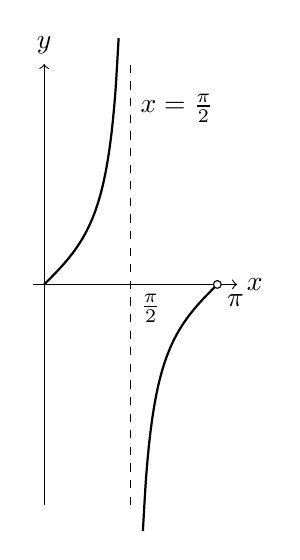
\begin{tikzpicture}[scale=0.7]
      % Grid and axes
      \draw[->] (-0.2,0) -- (3.5,0) node[right] {$x$};
      \draw[ ->] (0,-4) -- (0,4) node[above] {$y$};
      
      % Plotting tan(x)
      \draw[domain=0:0.5*pi-0.22,smooth,variable=\x,thick] plot ({\x},{tan(\x r)});
      \draw[domain=0.5*pi+0.22:pi,smooth,variable=\x,thick] plot ({\x},{tan(\x r)});
      
      % Asymptotes
      \draw[dashed] (pi/2,-4) -- (pi/2,4) node[pos=0.9,right] {$x=\frac{\pi}{2}$};
      
      % Labeling
      \node[below right] at (pi,0) {$\pi$};
      \node[below right] at (0.5*pi,0) {$\frac{\pi}{2}$};
      
      \draw[fill=white] (pi,0) circle [radius=2pt];
    \end{tikzpicture}
\end{center}
%\subsection{直线的方程}
%\subsubsection{直线方程的五种形式}
\begin{example}
    直线的倾斜角为\(\aa\in [\dfrac{\pi}{4},\dfrac{5\pi}{6})\)，求斜率的取值范围。
\end{example}

\begin{definition}[夹角与到角]
    \ 

    两相交直线的夹角 （两直线所成角）是指两直线所成的两对对顶角中，较小的一对角中一个的角；

一条直线\(l_1\)到另一条相交直线\(l_2\)的到角的定义为：\(l_1\)沿着与\(l_2\)的唯一交点逆时针旋转到第一次与\(l_2\)重合
时的有向角，将\(l_1\)称作到角的始边，\(l_2\)称作到角的终边。
\end{definition}
\begin{theorem}
    \begin{equation}
        \tan \theta=\tan \left(\alpha_{2}-\alpha_{1}\right)=\frac{\tan \alpha_{2}-\tan \alpha_{1}}{1+\tan \alpha_{1} \tan \alpha_{2}}=\frac{k_{2}-k_{1}}{1+k_{1} k_{2}}
    \end{equation}
\end{theorem}
\begin{theorem}
    \begin{equation}
        \tan \theta=\left|\frac{k_{1}-k_{2}}{1+k_{1} k_{2}}\right|
    \end{equation}
\end{theorem}
斜率可以非常方便地刻画直线的倾斜程度，但更多的要从题目中尝试去挖掘什么条件刻画了斜率的关系。
\begin{example}
    将直线\(l\)沿着\(y\)轴负方向平移\(a(a>0)\)个单位长度，再沿着\(x\)轴正方向平移\((a+1)\)个单位长度得到
    \(l'\)，则\(l\)的斜率为？
\end{example}
\begin{example}
    设\(A(x_1,y_1),B(x_2,y_2),C(x_3,y_3)\)是函数\(y=x^3\)图像上的任意三个不同的点，
    当\(A,B,C\)三点贡献的时候，求\(x_1+x_2+x_3\)的值。
\end{example}
而斜率不仅仅是刻画直线的倾斜程度，还可以由许多其他的应用。
\begin{theorem}
    \begin{equation}
        d=\sqrt{1+k^2}|x_1-x_2|
    \end{equation}
    \begin{equation}
        d=\sqrt{1+\frac{1}{k^2}}|y_1-y_2|
    \end{equation}
\end{theorem}
此定理的意义在于
\[|x_1-x_2|=\sqrt{(x_1-x_2)^2}=\sqrt{(x_1+x_2)^2-4x_1x_2}\]
\[|y_1-y_2|=\sqrt{(y_1-y_2)^2}=\sqrt{(y_1+y_2)^2-4y_1y_2}\]
最后能够化成关于斜率和韦达定理的形式。

此外，一些形如斜率定义式的式子，往往也可以使用斜率的集合意义求解

\begin{example}
    已知\(x,y\)满足\(y=\dfrac{1}{x}(\dfrac{1}{2}<x<2)\)，求$\dfrac{y+3}{x+2}$的取值范围。
\end{example}
\begin{exercise}
    试比较\(\dfrac{\ln 3}{2},\dfrac{\ln 4}{3},\dfrac{\ln 5}{4}\)的大小。
\end{exercise}
\begin{hint}考虑函数\(\ln (x+1)\)
\end{hint}

\begin{definition}[直线的方向向量与法向量]
    若直线的倾斜角为\(\theta\)，
    
    则直线的方向向量为\( \mathbf{t}\)以及与\( \mathbf{t}\)平行的各个非零向量；
    \begin{equation}
        \mathbf{t}=(\cos \theta,\sin \theta)
    \end{equation}
    直线的方向向量为\( \mathbf{b}\)以及与\( \mathbf{b}\)平行的各个非零向量。
    \begin{equation}
        \mathbf{b}=(\sin\theta,-\cos\theta)
    \end{equation}
\end{definition}
\begin{example}
    若直线\(l\)的一个方向向量为\(\mathbf{a}=\left(\sin\dfrac{\pi}{7},\cos\dfrac{\pi}{7}\right)\)，求直线的倾斜角和一个法向量。
\end{example}

在初中已经熟悉了
形如\(y=kx+b(k\neq 0)\)
的一次函数就是直线，如果允许\(k=0\)，就可以得到
平行于\(x\)轴的直线\(y=b\)。统一起来仍然是\(y=kx+b\)，只不过并不限制\(k\)的取值。
但是仍然有一种直线无法如此表示，即平行于$y$轴的直线\(x=a\)。两种直线在此并没有统一地表达，
原因也很容易看出来：\(y=kx+b\)的\(y\)前面没有参数，总是存在于表达式中，而\(x=b\)中没有\(y\)。

\begin{definition}[直线的一般式方程]
\begin{equation}
    Ax+By+C=0\quad(A^2+B^2\neq 0)
\end{equation}
\end{definition}
\(A^2+B^2\neq 0\)意味着\(A,B\)不同时为\(0\)，亦可以写作\((A,B)\neq (0,0)\)。
\begin{example}
    直线的方程$Ax+By+C=0(A^2+B^2\neq0)$中的\(A,B,C\)满足什么条件时，
直线分别具有如下性质：
\begin{minipage}[t]{0.45\textwidth}
    (1) 过坐标原点； \\
    (2) 与两条坐标轴都相交； \\
    (3) 与$x$轴无交点；
    \end{minipage}
    \hfill
    \begin{minipage}[t]{0.45\textwidth}
    (4) 与$y$轴无交点；\\
    (5) 与$x$轴垂直；\\
    (6) 与$y$轴垂直。
\end{minipage}
\end{example}

\begin{theorem}[一般式方程的方向向量与法向量]
    \ 

    直线\(Ax+By+C=0\)
    \begin{equation}
        \mathbf{t}=(B,-A)
    \end{equation}
    \begin{equation}
        \mathbf{b}=(A,B)
    \end{equation}
    
\end{theorem}


\begin{definition}[直线的斜截式方程]
    \begin{equation}
        y=kx+b
    \end{equation}
    \begin{equation}
        x=my+a
    \end{equation}
\end{definition}


\begin{definition}[直线的点斜式方程]
    \begin{equation}
        y-y_0=k(x-x_0)
    \end{equation}
\end{definition}
\begin{example}
    根据下列条件求直线的点斜式方程；
    
    (1)经过点$A(2,5)$，斜率为$4$；

(2) 经过点$B(-2,2)$，倾斜角为\(30\du \)。
\end{example}

\begin{example}
    已知$P$是直线上一点，且\(\mathbf{t}\)是直线的一个方向向量，
    \(\mathbf{b}\)是直线的一个方向向量，分别根据下列条件求直线的方程：

$(1)\ P(3,5),\ \mathbf{t}=(1,2)$；      

$(2)\ P(1,2),\ \mathbf{b}=(3,4)$。
\end{example}




\begin{definition}[直线的两点式方程]
    
    \begin{equation}
        \frac{y-y_{1}}{y_{2}-y_{1}}=\frac{x-x_{1}}{x_{2}-x_{1}},
    \end{equation}
\end{definition}

\begin{example}
    已知直线经过点$A(2,1),B(3,3)$，求直线的方程，并求直线的截距。
\end{example}
\begin{definition}[直线的截距式方程]
    \begin{equation}
        \frac{x}{a}+\frac{y}{b}=1\quad (ab\neq 0)
    \end{equation}
\end{definition}

\begin{example}
    已知直线\(l\)过点\((3,4)\)，且直线在\(x\)轴和\(y\)轴上的截距相等。求直线的方程。
\end{example}
\begin{exercise}
    已知直线\(l\)过点\(A(-4,-2)\)，且\(A\)是直线\(l\)被两坐标轴截得的线段中线，求直线\(l\)的方程。
\end{exercise}

\begin{theorem}
    直线\(l_1:A_1x+B_1y+C_1=0,l_2:A_2x+B_2y+C_2=0\)，则过\(l_1,l_2\)交点\(P\)的直线方程可写作
    \begin{equation}
        \lambda(A_1x+B_1y+C_1)+\mu(A_2x+B_2y+C_2=0)=0\quad (\lambda^2+\mu^2\neq 0)
    \end{equation}
\end{theorem}

\begin{example} 求出下列直线过的定点。

    （1）\(y=kx+b, b=2k+1\)；
    
    （2）\((2k+1)x+ky+5=0\)。
\end{example}
\clearpage
\subsection{直线的位置关系}
平面上两条直线应该有两种位置关系：平行和相交，当然有时候会把重合算作第三种关系。而其中的
相交还有特殊情况——垂直。接下来使用斜截式和一般式研究直线的位置关系。
\begin{theorem}
    直线\(l_1:A_1x+B_1y+C_1=0,l_2:A_2x+B_2y+C_2=0\)
\begin{enumerate}[(1)]
    \item 平行
    \begin{equation}
        \frac{A_1}{A_2}=\frac{B_1}{B_2}\neq \frac{C_1}{C_2}
    \end{equation}
    \item 重合
    \begin{equation}
        \frac{A_1}{A_2}=\frac{B_1}{B_2}=\frac{C_1}{C_2}
    \end{equation}
    \item 相交
    \begin{equation}
        \frac{A_1}{A_2}\neq \frac{B_1}{B_2}
    \end{equation}
    \item 垂直
    \begin{equation}
        A_1A_2+B_1B_2=0
    \end{equation}
\end{enumerate}
\end{theorem}


\begin{corollary}
    直线\(l_1:y=k_1+b_1,l_2:y=k_2x+b_2\)
\begin{enumerate}[(1)]
    \item 平行
    \begin{equation}
        k_1=k_2,b_1\neq b_2
    \end{equation}
    \item 重合
    \begin{equation}
        k_1=k_2,b_1= b_2
    \end{equation}
    \item 相交
    \begin{equation}
        k_1\neq k_2
    \end{equation}
    \item 垂直
    \begin{equation}
        k_1k_2=-1
    \end{equation}
\end{enumerate}
\end{corollary}
\begin{example}
\ 

（1）已知点 $ A(m, 3), B(2 m, m+4), C(m+1,2), D(1,0) $, 且直线 $ A B $ 与直线 $ C D$  平行, 求实数  $m $ 的 值  ；

（2）已知经过点 $ A(-2,0) $ 和点  $B(1,3 a)$  的直线  $l_{1} $ 与经过点 $ P(0,-1)$ 和点  $Q(a,-2 a)$  的直线 $ l_{2} $ 互相垂直, 求实数  $a$  的值为？
\end{example}
\begin{exercise}
    已知直线\(l_1:y=2x+3a,l_2:y=(a^2+1)x+3\)，若\(l_1\pll l_2\)求m的值。
\end{exercise}


\begin{att}
    要时刻注意直线斜率存在与否，以及倾斜角相同的直线是否重合。
\end{att}
\begin{example}
    已知集合\(A=\{(x,y)|\dfrac{y-3}{x-2}=a+1\}\),\(B=\{(x,y)|(a^2-1)x+(a-1)y=15\}\)，若
    \(A\cup B=\varnothing \)，则求\(a\)可能的值。
\end{example}

\begin{definition}[平行直线束]
    \begin{equation}
        y=k_0x+b
    \end{equation}
    \begin{equation}
        A_0x+B_0y+C=0
    \end{equation}
\end{definition}
\begin{definition}[过定点的直线束]
    \begin{equation}
        y-y_0=k(x-x_0)
    \end{equation}
\end{definition}
\begin{example}
    已知直线\(l\)与直线\(y=\dfrac{1}{2}x+4\)互相垂直，直线\(l\)与直线\(y=x+6\)在y轴上截距相等，试求直线
    \(l\)方程。
\end{example}
\clearpage
\subsection{直线相关的距离公式}
\begin{theorem}
    \begin{equation}
          d=\frac{|Ax_0+By_0+C|}{\sqrt{A^2+B^2}}
    \end{equation}
\end{theorem}
\begin{exercise}
    求点\(P_0(-1,2)\)到下列直线的距离\(d\)：
    \begin{enumerate}[(1)]
        \setlength{\itemsep}{-\itemsep}
        \item \(2x+y-10=0\)；
        \item \(y-3=0\)；
        \item \(x+2=0\)。
    \end{enumerate}
\end{exercise}
\begin{example}
    已知直线 $ l: k x+y+2-k=0 $ 过定点$  M$ ,点 $ P(x, y)$  在直线 $ 2 x-y+1=0$  上, 试求线段$  |M P| $ 的最小值。
\end{example}
\begin{theorem}
    \begin{equation}
          d=\frac{|C_1-C_2|}{\sqrt{A^2+B^2}}
    \end{equation}
\end{theorem}
\begin{exercise}
    求直线\(x+y-1=0\)与直线\(2x+2y+5=0\)之间的距离。
\end{exercise}
在初中就已经熟悉了一点\(P(x,y)\)关于原点、\(x\)轴、\(y\)轴对称后的坐标，后两者可以简单记忆为“关于谁，谁不变”。
\begin{character}
    \ 

 点 $ P\left(x_{0}, y_{0}\right)$ 关于原点的对称点为 $P^{\prime}\left(-x_{0},-y_{0}\right)$ ；

 点  $P\left(x_{0}, y_{0}\right)$  关于  x  轴的对称点为 $ P^{\prime}\left(x_{0},-y_{0}\right)$ ；

  点 $ P\left(x_{0}, y_{0}\right)$  关于  y  轴的对称点为  $P^{\prime}\left(-x_{0}, y_{0}\right) $。
\end{character}

但是如果这个点不再是原点，而是一般的点\((m,n)\)呢？直线也变成了一般式\(Ax+By+C=0\)。
\begin{example}
    求点\(P(x_0,y_0)\)关于点M\((m,n)\)的对称点。
\end{example}
\begin{example}
    求点\(P(x_0,y_0)\)关于直线\(l:Ax+By+C=0\)的对称点。
\end{example}
\begin{example}
    求线\(l:Ax+By+C=0\)关于点M\((m,n)\)的对称点。
\end{example}

\begin{example}
    求线\(l:Ax+By+C=0\)关于点线\(l_0:ax+by+c=0\)的对称点。
\end{example}






\clearpage
\review

\clearpage

\hw
\begin{homework}
    判断下列有关直线方程的命题的真假。
    \begin{enumerate}[(1)]
        \setlength{\itemsep}{-\itemsep}
        \item 平面上任何一条直线都可以用一个关于\(x,y\)的二元一次方程\(Ax+By+C=0(A^2+B^2\neq 0)\)表示。
        \item 当\(C=0\)时，方程\(Ax+By+C=0(A^2+B^2\neq 0)\)表示的直线过原点。
        \item 当\(A=0,B\neq 0,C\neq 0\)时，方程\(Ax+By+C=0\)表示的直线与\(x\)轴平行。
        \item 任何一条直线的一般式都能与其他四种形式互化。
        \item 斜率相等的直线可以用\(\dfrac{x}{a}+\dfrac{y}{a}=1\)表示。
        \item \(x+my-2=0(m\in\mathbb{R})\)能表示平行于\(y\)轴的直线。
        \item 记过点\(P(1,1)\)，倾斜角为\(\theta\)的直线方程为\(y-1=\tan\theta(x-1)\)。
        \item 过\((x_1,y_1),(x_2,y_2)\)两点的直线方程为\(\dfrac{y-y_{1}}{y_{2}-y_{1}}=\dfrac{x-x_{1}}{x_{2}-x_{1}}\)
    \end{enumerate}
\end{homework}
\begin{homework}
已知$G(-1,0)$为正方形的中心，且这个正方形的一条边所在的直线方程为
$x-3y-5=0$，求这个正方形其他三条边所在的直线的方程。

\end{homework}
\begin{homework}
    已知直线\(l\)经过点$P(2,1)$，且$A(2,3),B(4,—5)$两点到直线的距离相等，求直线\(l\)的方程。
\end{homework}
\begin{homework}

\end{homework}
\begin{homework}求证：
    
    点$  P\left(x_{0}, y_{0}\right)$  关于直线 $ y=x $ 的对称点为 $ P^{\prime}\left(y_{0}, x_{0}\right)$ ；

 点  $P\left(x_{0}, y_{0}\right) $ 关于直线 $ y=-x $ 的对称点为 $ P^{\prime}\left(-y_{0},-x_{0}\right) $；

 点  $P\left(x_{0}, y_{0}\right) $ 关于直线 $ x=m $的对称点为 $ P^{\prime}\left(2 m-x_{0}, y_{0}\right) $；

 点 $ P\left(x_{0}, y_{0}\right) $ 关于直线 $ y=n $ 的对称点为 $ P^{\prime}\left(x_{0}, 2 n-y_{0}\right) $。
\end{homework}
\begin{homework}求证：

直线 $ l: A x+B y+C=0 $ 关于 $ x  $轴的对称直线为  $l^{\prime}: A x+B(-y)+   C=0 .$

直线 $ l: A x+B y+C=0 $ 关于 $ y$  轴的对称直线为 $ l^{\prime}: A(-x)+B y+   C=0 .$

直线 $ l: A x+B y+C=0  $关于直线$  y=x $ 的对称直线为  $l^{\prime}: B x+   A y+C=0 .$

直线 $ l: A x+B y+C=0 $ 关于直线$  y=-x $ 的对称直线为 $ l^{\prime}: A(-y)+   B(-x)+C=0 .$
\end{homework}
\begin{homework}
    
\end{homework}
\begin{homework}
    
\end{homework}
\begin{homework}
    
\end{homework}
\begin{homework}
    
\end{homework}
\begin{homework}
    
\end{homework}
\begin{homework}
    
\end{homework}
\begin{homework}
    
\end{homework}
\begin{homework}
    
\end{homework}
\begin{homework}
    
\end{homework}

\clearpage


\section{圆}
\subsection{圆的方程}
\begin{definition}
    圆是平面内到一定点的距离等于定长的点的集合。
\end{definition}
\begin{theorem}[圆的标准方程]
    \begin{equation}
        (x-a)^2+(y-b)^2=r^2
    \end{equation}
\end{theorem}

\begin{corollary}[圆与点的位置关系]
    判断一个点在圆内、圆上还是圆外的方法：设\(\odot C\)的圆心为$C(a,b)$，半径为\(r>0\)，则
    
    点$(x_0,y_0)$在\(\odot C\)内\(\Leftrightarrow   (x_0-a)^2+(y_0-b)^2>r^2\)；

    点$(x_0,y_0)$在\(\odot C\)上\(\Leftrightarrow   (x_0-a)^2+(y_0-b)^2=r^2\)；

    点$(x_0,y_0)$在\(\odot C\)外\(\Leftrightarrow   (x_0-a)^2+(y_0-b)^2<r^2\)。
\end{corollary}
\begin{example}
    已知圆\(C\)的方程为\(f(x,y)=0\)，点\(A(x_0,y_0)\)在圆外，点\(B(x',y')\)在圆上，
    则求\(f(x,y)-f(x_0,y_0)+f(x',y')=0\)表示的曲线。
\end{example}
\begin{exercise}
    观察下列方程，写出方程对应的轨迹。如果是圆，请指出圆心和半径。
    \begin{enumerate}[(1)]
        \item \[(x+1)^2+(y-3)^2=2\]
        \item \[x^2+(y-4)^2=-4\]
        \item \[(x-4)^2+(y+2)^2=0\]
    \end{enumerate}
\end{exercise}

\begin{example}
    根据下列条件，求圆的标准方程：

   (1)圆心在点$C(-2,1)$，且过点$A(2,2)$；

   (2) 过点$(0,1)$和点$(2,1)$，半径为\(\sqrt{5}\)。

   (3) 设\(\odot C\)的圆心$C$在直线$l$：$2x-7y+8=0$上，$A(6,0),\ B(1,5)$都是$C$上的点。
\end{example}
\begin{theorem}[垂径定理]
    垂直于弦的直径平分弦且平分这条弦所对的两条弧；
    平分弦（非直径）的直径垂直于这条弦，并且平分这条弦所对的两条弧；
    垂直平分弦的弦一定是直径，且平分另一条弦所对的两条弧。

    实际上在一个圆中有两条弦，若其中一条弦满足下列五个条件中的两个，则必定满足其他三个条件：

    （1）平分另一条弦所对的优弧
    
    （2）平分另一条弦所对的劣弧
    
    （3）平分另一条弦
    
    （4）垂直于另一条弦
    
    （5）过圆心（或是直径）

\end{theorem}
如果将圆的标准方程展开
\begin{align*}
    (x-a)^2+(y-b)^2&=r^2\\
    x^2-2ax+a^2+y^2-2by+b^2&=r^2\\
    x^2+y^2-2ax-2by+(a^2+b^2-r^2)&=0\\
\end{align*}
得到类似这样的式子，相比配方好的标准式，它们更符合我们一般认知中的方程。
\begin{theorem}[圆的一般方程]
    \begin{equation}
        x^2+y^2+Dx+Ey+F=0
    \end{equation}
\end{theorem}
\begin{jie}
    \begin{align*}
        x^2+y^2+Dx+Ey+F&=0\\
        x^2+Dx+\frac{D^2}{4}+y^2+Ey+\frac{E^2}{4}&=\frac{D^2}{4}+\frac{E^2}{4}-F\\
        (x+\frac{D}{2})^2+(y+\frac{E}{2})^2&=\frac{D^2}{4}+\frac{E^2}{4}-F\\
    \end{align*}
    \[r=\frac{\sqrt{D^2+E^2-4F}}{2}\]
\end{jie}

\begin{example} 判断下列方程是否是圆的方程，如果是，写出圆的圆心坐标与平径；如果不是，说明理由。

    $(1)  x^{2}+y^{2}+4 x-6 y-12=0 $；

$(2)  4 x^{2}+4 y^{2}-8 x+4 y-15=0 $；

$(3)  x^{2}+y^{2}-6 x+10=0 $；

$(4)x^{2}+y^{2}+4x+2y+5=0$.
\end{example}
圆系

\begin{example}
    求经过\(A,B,C\)三点的圆的方程：

    \((1)A(0,0),B(2,0),C(0,2)\)

    \((2)A(5,1),B(7,-3),C(2,-8)\)
\end{example}
\begin{jie}
    \ 

    $(1)$

    \((2)\)
    \begin{way1}
        
    \end{way1}
    \begin{way2}
        设圆的方程为\((x-a)^2+(y-b)^2=r^2\)
    \end{way2}
    \begin{way3}
        设圆的方程为\(x^2+y^2+Dx+Ey+F=0\)
    \end{way3}
\end{jie}
\begin{theorem}
    二元二次方程\begin{equation}
        Ax^2+By^2+Cxy+Dx+Ey+F=0
    \end{equation}
    在平面直角坐标系中对应的曲线一定是
    圆、椭圆、双曲线、抛物线、两条（相交、平行或重合的）直线、一个点、空集之一。
\end{theorem}
\begin{theorem}
    $x^{2}+y^{2}+D_{1} x+E_{1} y+F_{1}=0$ ，$C_{2}: x^{2}+y^{2}+D_{2} x+E_{2} y+F_{2}=0$

    \begin{equation}
        \lambda(x^{2}+y^{2}+D_{1} x+E_{1} y+F_{1})+\mu(x^{2}+y^{2}+D_{2} x+E_{2} y+F_{2})=0
    \end{equation}
\end{theorem}
\clearpage
\subsection{直线、圆的位置关系}
\begin{definition}[直线与圆的位置关系]
    如图\ref{图圆与直线相交}所示，直线与圆有两个公共点
时，称直线与圆相交，且称直线为圆的割线；
如图\ref{图圆与直线相切}所示，直线与圆只有一个公共点时，称直线与圆相切，且称直线为圆的切线，称公共点为切点；
如图\ref{图圆与直线相离}所示，直线与圆没有公共点时，称直线与圆相离。
\end{definition}
\begin{figure}[h]
    \centering
    \begin{subfigure}[b]{0.3\textwidth}
        \centering
        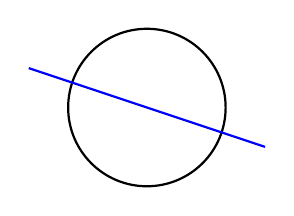
\begin{tikzpicture}
            \draw[thick, black] (0,0) circle (1cm); % 圆
            \draw[thick, blue] (-1.5,0.5) -- (1.5,-0.5); % 相交直线
        \end{tikzpicture}
        \caption{相交}
        \label{图圆与直线相交}
    \end{subfigure}
    \hfill
    \begin{subfigure}[b]{0.3\textwidth}
        \centering
        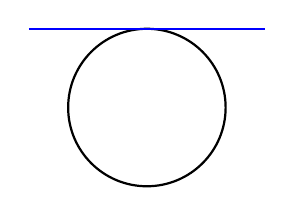
\begin{tikzpicture}
            \draw[thick, black] (0,0) circle (1cm); % 圆
            \draw[thick, blue] (-1.5,1) -- (1.5,1); % 相切直线
        \end{tikzpicture}
        \caption{相切}
        \label{图圆与直线相切}
    \end{subfigure}
    \hfill
    \begin{subfigure}[b]{0.3\textwidth}
        \centering
        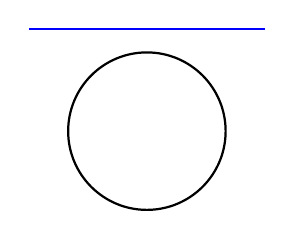
\begin{tikzpicture}
            \draw[thick, black] (0,0) circle (1cm); % 圆
            \draw[thick, blue] (-1.5,1.3) -- (1.5,1.3); % 相离直线
        \end{tikzpicture}
        \caption{相离}
        \label{图圆与直线相离}
    \end{subfigure}
    \caption{圆与直线的关系示意图}
\end{figure}

\begin{theorem}
    如果圆的的半径为\(r\)，圆心到直线的距离为\(d\)，则

    \centering     直线与圆相交\(\Leftrightarrow d<r\)；

    \centering     直线与圆相切\(\Leftrightarrow d=r\)；

    \centering     直线与圆相离\(\Leftrightarrow d>r\)。
\end{theorem}
\begin{jie}
    
\end{jie}




\begin{example}
    判断直线\(l:y=-x+5\)与圆\(C:x^2+y^2=12\)的位置关系。
\end{example}
\begin{exercise}
    
\end{exercise}
\begin{jie}
    
    \qed
\end{jie}

在这里阐释一下相切的意义。从初中到现在，一直都是使用交点个数来定义“相交”、“相切”和“相离”。
但是这个定义并不完美，在初中我们就遇到了抛物线和其对称轴的情况——直线和曲线有一个交点，却很难让人觉得这是
相切关系。在此应该用更加现代的观点重新审视“相切”这一词。







这种定义相切的方法还有很多细节要说，但是这不是这节的重点。仅仅是想解释：使用切点个数来定义相切和使用这种动态
的方法定义相切有本质的区别。
在此并没有给出一个确切的方法来计算这种动态过程产生的切线，我们将在第\ref{导数的初步认识}章
学习导数的相关知识，了解这种切线定量的计算方法。
因此暂时还是使用交点的个数来定义相切——至少在这几章内不会出现大问题。




\begin{example}根据已知条件求切线方程：

    （1）已知点\(M(1,2)\)和圆\(x^2+(y-1)^2=2\)，求在点\(M\)的圆的切线；

    （2）已知点\(N(1,1)\)和圆\((x-3)^2+(y+1)^2=4\)，求过点\(M\)的圆的切线。
\end{example}
区分“在某处的切线”和“过某处的切线”。
\begin{theorem}[切线长定理]
    从圆外一点引圆的两条切线，它们的切线长相等，且这点与圆心的连线平分两条切线的夹角。
    \begin{definition}[切线长]
        经过圆外一点做圆
        的切线，这点和切点之间的线段的长叫做这点到圆的切线长。
    \end{definition}
\end{theorem}
\begin{theorem}\label{圆的切线方程定理}
    圆\(x^2+y^2=r^2\)在点\((x_0,y_0)\)处的切线方程为
    \begin{equation}\label{圆的切线方程}
        x_0x+y_0y=r^2
    \end{equation}
\end{theorem}
\begin{corollary}\label{圆的切线方程推论}
    \ 

    圆\((x-a)^2+(y-b)^2=r^2\)在点\((x_1,y_1)\)处的切线方程为
    \begin{equation}
        (x_1-a)(x-a)+(y_1-b)(y-b)=r^2
    \end{equation}

    圆\(x^2+y^2+Dx+Ey+F=0\)在点\((x_2,y_2)\)处的切线方程为
    \begin{equation}
        x_2x+y_2y+D\frac{x_2+x}{2}+E\frac{y_2+y}{2}+F=0
    \end{equation}
\end{corollary}
定理\ref{圆的切线方程定理}、推论\ref{圆的切线方程推论}给了一个极强的条件——知道了曲线上的点，可以直接写出在这一点
的切线方程。那如果这个点不在曲线上，方程\ref{圆的切线方程}有什么含义呢？

\begin{theorem}
    若点\(x_0,y_0\)在圆\(x^2+y^2=r^2\)外，则方程\[x_0x+y_0y=r^2\]表示切点弦所在直线的方程。
\end{theorem}









\begin{example}
    已知圆\(C:x^2+y^2+Dx+Ey+F=0\)和点\(M(x_0,y_0)\)为圆外一点，求\(M\)到圆\(C\)的切线长。
\end{example}
\begin{jie}
    \[(x_0+\frac{D}{2})^2+(y_0+\frac{E}{2})^2=l^2+\frac{D^2}{4}+\frac{E^2}{4}-F\]

\qed
\end{jie}

\begin{example}
    已知直线 $ l: x+y+2=0  $与圆$  C: x^{2}+y^{2}=9$  相交于 $ A, B$  两点.

    （1）求线段 $ A B $ 的长；

    （2） 求线段  $A B $ 中点的坐标。
\end{example}

\begin{example}
    若  $P(x, y) $ 是圆 $ C:(x-3)^{2}+y^{2}=1  $上的任意一点, 求 $ P(x, y) $ 到直线 $ x-y+1=0 $ 的距离的最大值和最小值。
\end{example}

\begin{definition}
    
\end{definition}
\begin{theorem}
xxxxx
\vspace*{-0.3cm}
    \begin{align*}
        \text{两个圆外离} & \Leftrightarrow d > r_{1} + r_{2} \\
        \text{两个圆外切} & \Leftrightarrow d = r_{1} + r_{2} \\
        \text{两个圆相交} & \Leftrightarrow \left| r_{1} - r_{2} \right| < d < r_{1} + r_{2} \\
        \text{两个圆内切} & \Leftrightarrow d = \left| r_{1} - r_{2} \right| \\
        \text{两个圆内含} & \Leftrightarrow d < \left| r_{1} - r_{2} \right| \\
    \end{align*}
    \vspace*{-1.4cm}
\end{theorem}
\begin{exercise}
    分别指出下列两圆的位置关系 (外离、外切、相交、内切、内含):

(1) $ x^{2}+y^{2}-4 x-6 y+9=0 \text{和}   x^{2}+y^{2}+12 x+6 y-19=0 ;$

(2) $ x^{2}+y^{2}+2 x-2 y-2=0 \text{和}  x^{2}+y^{2}-4 x-6 y-3=0 .$
\end{exercise}

\begin{theorem}
    若两圆  $C_{1}: x^{2}+y^{2}+D_{1} x+E_{1} y+F_{1}=0, C_{2}: x^{2}+y^{2}+D_{2} x+E_{2} y+F_{2}=0  $
    相交于 $ A, B  $两点，则直线 $ A B  $的方程为 
    \begin{equation}\label{根轴方程}
         \left(D_{1}-D_{2}\right) x+\left(E_{1}-E_{2}\right) y+F_{1}-F_{2}=0 
    \end{equation}

    若两圆相切，则方程\ref{根轴方程}是经过两圆切点的公切线；

    \begin{definition}[根轴]
        在平面上任给两不同心的圆，则到两圆切线长相等的点的集合是一条直线，这条线称为这两个圆的根轴。
    \end{definition}

    方程\ref{根轴方程}（在有意义的情况下）总是两圆的根轴。
\end{theorem}
\begin{exercise}
     若圆 $x^{2}+y^{2}=1 $ 与 $ x^{2}+y^{2}+2 x-2 y=0 $ 相交于$  A ,B $ 两点，求直线  $A B $的方程。
\end{exercise}

接下来研究一下两个圆公切线的数量及求法。

\begin{theorem}[切线的数量]
\ 

    \begin{center}
        \begin{minipage}{0.3\textwidth} % 设置 minipage 的宽度，例如 50% 的文本宽度
          \raggedright % 使文本左对齐
          两个圆外离：四条切线

       两个圆外切：三条切线

       两个圆相交：两条切线

       两个圆内切：一条切线

      两个圆内含：零条切线
        \end{minipage}
      \end{center}
\end{theorem}

\begin{example}
 求圆 $C_1:x^{2}+y^{2}=1 $和$C_2:(x-3)^{2}+(y-4)^{2}=16 $的公切线方程。
\end{example}



\clearpage

%\subsubsection{Apollonius圆}


\clearpage
\review
\clearpage
\hw
\begin{homework}
    若 $ P(x, y) $ 是圆 $ C:(x-1)^{2}+y^{2}=\dfrac{1}{4}$  上的任意一点, 求 $ P(x, y) $ 到原点的距离的最大值和最小值.
\end{homework}
\begin{homework}
    求圆  $x^{2}+y^{2}+2 x-2 a y-4=0(a \in \mathbb{R})$  的半径的最小值.
\end{homework}
\begin{homework}
    
\end{homework}
\begin{homework}
    
\end{homework}
\begin{homework}
    
\end{homework}
\begin{homework}
    
\end{homework}
\begin{homework}
    
\end{homework}
\begin{homework}
    
\end{homework}
\begin{homework}
    
\end{homework}
\clearpage

\section{线性规划初步*}
\subsection{二元一次不等式的几何意义}
\clearpage
\subsection{线性规划的应用}
要讲完一些解析几何
\clearpage

\chapter{解析几何（二）}

\clearpage

\section{椭圆}
\subsection{椭圆的方程与性质}
椭圆给人的直观感受无非就是扁了的圆，但是这如何用数学语言去刻画呢？
联想到三角函数\(y=\sin x\)与\(y=A\sin(\omega x)\)，其中参数\(A\)和$\omega$都是对函数的
拉伸或压缩。由此可以给出椭圆的一个简单的定义：
\begin{definition}[椭圆的第零定义]
    给一个单位圆\(x^2+y^2=1\)，做伸缩变换
    \[ \left\{
        \begin{array} { l } 
        x'=a x\\
        y'=b y
        \end{array}
    \right.\]
    则变换后的方程
    \[\frac{x^2}{a^2}+\frac{y^2}{b^2}=1\]在平面直角坐标系的轨迹中为椭圆。
\end{definition}

\begin{definition}[椭圆的第一定义]
    到平面内两定点距离之和为定值（距离之和大于两定点间距离）的点的集合为椭圆。其中，称两个定点为椭圆的两个焦点(focal point)；
    定点之间的距离称为椭圆的焦距(focal length)。
\end{definition}
展开来讲，平面上首先应该有两个定点称作焦点，记为\(F_1,F_2\)，并设\(|F_1F_2|=2c\)。
再有一个定值，设之为\(2a\)，且\(2a>2c\)。那么椭圆就是下面的集合：
\[\{P\in \mathbb{R}^2||PF_1|+|PF_2|=2a\}\]
\begin{theorem}[椭圆的标准方程]
    \begin{equation}
        \frac{x^2}{a^2}+\frac{y^2}{b^2}=1 \quad (a>b>0)
    \end{equation}
    \begin{equation}
        a^2=b^2+c^2
    \end{equation}
    \begin{equation}
        \frac{y^2}{a^2}+\frac{x^2}{b^2}=1 \quad (a>b>0)
    \end{equation}
\end{theorem}
\begin{proof}
    设焦距为\(2c\)，不妨把它放置在\(x\)轴上，设为\(F_1(-c,0), F_2(c,0)\)。再设
    到两个焦点的距离之和为\(2a\)。
    \begin{way1}考虑共轭根式
        
    \end{way1}

    \begin{way2}考虑将根号分布在等式两侧处理。
        
    \end{way2}
    \qed
\end{proof}
在推导完椭圆的方程之后，一个自然的问题是：条件\(2a>2c\)起到了什么样的作用？其实在上述推导过程中可以窥见一点：
\begin{corollary}
    \(a=c\) 线段\(F_1F_2\)

    \(a<c\) 空集
\end{corollary}
\begin{example}
    判断下列方程所代表的椭圆焦点是在\(x\)轴上还是\(y\)轴上。并指出标准方程中的\(a,b,c\)。
\end{example}
\begin{example}
    求满足下列条件的椭圆的标准方程：
\end{example}
\begin{exercise}
    满足下列条件的点的轨迹是椭圆吗？如果是，写出标准方程，并计算出标准方程中的\(a,b,c\)；如果不是，说明理由。
\end{exercise}

\begin{example}
    
\end{example}
%\subsubsection{椭圆的标准方程}
%\subsubsection{椭圆的几何性质}
\begin{character}[椭圆的性质]
\begin{enumerate}[(1)]
    \item 有界性
    \item 对称性
    \item 顶点
\end{enumerate}
\end{character}
\begin{definition}[离心率]
    \begin{equation}
        e=\frac{c}{a}
    \end{equation}
\end{definition}
\begin{theorem}[椭圆的离心率]
    \begin{equation}
        e\in (0,1)
    \end{equation}
    椭圆的离心率越接近\(0\)则越圆；椭圆的离心率越接近\(1\)越扁。
\end{theorem}

\begin{definition}[通径]
    
\end{definition}

\clearpage












\subsection{椭圆的其他定义}
\begin{definition}[椭圆的第二定义]
    到定点的距离与到定直线的距离的比值为一个定值\(e(\in(0,1))\)的点的轨迹为椭圆。
    该定点称为椭圆的焦点，定直线称为椭圆的准线，\(e\)称为离心率。
\end{definition}

\begin{jie}
    过焦点做准线的垂线作为\(x\)轴，以焦点指向准线的方向为正方向。选取合适的\(y\)轴，使得准线的方程为
    \(x=\dfrac{a^2}{c}\)，焦点的坐标是\((c,0)\)。
    
    由题意列式：
       \[ \frac{\sqrt{(x-c)^2+y^2}}{\left|x-\frac{a^2}{c}\right|}=e\]
两侧平方，将分母移到右边并展开括号得
\[x^2-2cx+c^2+y^2=e^2\left(x^2-2\frac{a^2}{c}x+\frac{a^4}{c^2}\right)\]    
移项得
\[\left(1-e^2\right)x^2+y^2+\left(2e^2\frac{a^2}{c}-2c\right)x=e^2\frac{a^4}{c^2}-c^2\]
取\(e=\dfrac{c}{a},\ b^2=a^2-c^2\)，则得到
\vspace*{-0.5cm}
\begin{align*}
    \frac{b^2}{a^2}x^2+y^2&=b^2\\
    \frac{x^2}{a^2}+\frac{y^2}{b^2}&=1\\
\end{align*}
这恰好就是椭圆的标准方程。
\end{jie}
\begin{character}
    \ 
    
    准线

    焦准距
\end{character}

\begin{theorem}[焦半径公式]
    
\end{theorem}









\clearpage
%\subsection{椭圆的光学性质}
\clearpage

\section{双曲线}
\subsection{双曲线的方程与性质}
\begin{definition}[双曲线的第一定义]
    到平面内两定点距离之差的绝对值为定值的点的集合为椭圆（如果不是空集）。其中，称两个定点为双曲线的两个焦点；
    定点之间的距离称为双曲线的焦距。
\end{definition}
\begin{theorem}[双曲线的标准方程]
    \begin{equation}
        \frac{x^2}{a^2}-\frac{y^2}{b^2}=1 
    \end{equation}
    \begin{equation}
        c^2=a^2+b^2
    \end{equation}
    \begin{equation}
        \frac{y^2}{a^2}-\frac{x^2}{b^2}=1 
    \end{equation}
\end{theorem}
\begin{example}
    求满足下列条件的双曲线的标准方程：
\end{example}

\begin{character}[双曲线的性质]
\begin{enumerate}[(1)]
    \item 无界性
    \item 对称性
    \item 顶点
\end{enumerate}
\end{character}

\begin{theorem}[双曲线的离心率]
    \begin{equation}
        e\in (1,\infty)
    \end{equation}

\end{theorem}

\begin{definition}[通径]
    
\end{definition}

%\subsubsection{双曲线的标准方程}
\clearpage
%\subsubsection{双曲线的几何性质}
\clearpage
\subsection{双曲线的其他定义}
\clearpage
%\subsection{双曲线的光学性质}
\clearpage
\subsection{几种常见的双曲线}
\clearpage

\section{抛物线}
\subsection{抛物线的方程与性质}

\begin{example}
    已知抛物线\(y^2=4x\)的焦点为\(F\)，\(\tri ABC\)的三个顶点都在抛物线上，且\(F\)
    为\(\tri ABC\)的重心，求\(|AF|+|BF|+|CF|\)和\(|AF|^2+|BF|^2+|CF|^2\)的值。
\end{example}









\subsubsection{抛物线的标准方程}
\clearpage
\subsubsection{抛物线的几何性质}
\clearpage
%\subsection{抛物线的光学性质}
\clearpage

\section{圆锥曲线的联立}
\subsection{位置关系}

\begin{theorem}
    椭圆\(C:\dfrac{x^2}{a^2}+\dfrac{y^2}{b^2}=1\)，\(P(x_0.y_0)\)为\(C\)上一点。则过\(P\)点的切线方程为
    \begin{equation}
        \dfrac{x_0x}{a^2}+\dfrac{y_0y}{b^2}=1
    \end{equation}
\end{theorem}
\begin{corollary}
    椭圆\(C:\dfrac{x^2}{a^2}+\dfrac{y^2}{b^2}=1\)，\(P(x_0.y_0)\)为\(C\)外一点。则过\(P\)点对应的切点弦方程为
    \begin{equation}
        \dfrac{x_0x}{a^2}+\dfrac{y_0y}{b^2}=1
    \end{equation}
\end{corollary}
















\clearpage
\subsection{韦达定理}
\subsubsection{弦长}
\clearpage
\subsubsection{向量关系}
\clearpage
\subsubsection{斜率关系}
\clearpage
\subsubsection{焦半径}



\chapter{解析几何（三）}
\clearpage
\section{几种常见的坐标系*}
\subsection{极坐标系}
\subsubsection{基础概念与相互转化}
\clearpage
\subsubsection{常见的极坐标方程}
\clearpage
\subsection{球坐标系与柱坐标系}
\clearpage



\section{参数方程*}
\subsection{参数方程的概念}
\clearpage
\subsection{圆锥曲线的参数方程}
\begin{theorem}[圆的参数方程]
    以 \( O(x_0, y_0) \)为圆心，\(r\)为 半径的 \( \bigodot O  \) 的参数方程为
    \[\left\{
    \begin{gathered}
        x = x_0 + r \cos \alpha, \\
        y = y_0 + r \sin \alpha,
    \end{gathered}\right.
    \ (\alpha\text{为参数})
    \]
\end{theorem}


\begin{example}
    已知 \(x^2 + y^2 - 2y - 3 = 0\)，求 \(2x^2 + 2y^2 - 3x\) 的取值范围。
\end{example}

\begin{example}
    求\(f(x)=\dfrac{\sin x-3}{\cos x -1}\)的值域。
\end{example}

\begin{example}
    已知\(P\)是\(\bigodot C:(x-1)^2+y^2=1\)上一动点，两定点\(M(-1,0), N(0,-1)\)，求\(|PM|^2+|PN|^2\)的取值范围。
\end{example}
\begin{exercise}
    已知\(P\)是\(\bigodot C:x^2+y^2=4\)上一动点，两定点\(A(0,-4), B(2,0)\)，求\(\dfrac{|PB|}{|PA|}\)的取值范围。
\end{exercise}
\begin{theorem}[椭圆的参数方程]
标准方程为\(\dfrac{x^2}{a^2}+\dfrac{y^2}{b^2}=1\)的椭圆的参数方程为
    \[\left\{
    \begin{gathered}
        x = a \cos \alpha, \\
        y = b \sin \alpha,
    \end{gathered}\right.
    \ (\alpha\text{为参数})
    \]
\end{theorem}
\begin{corollary}[椭圆参数方程中参数的几何意义]
    
\end{corollary}
\begin{example}
    已知椭圆 \(\dfrac{x^2}{25} + \dfrac{y^2}{9} = 1\)，直线 \(l: 4x - 5y + 40 = 0\)。椭圆上是否存在一点，它到直线 \(l\) 的距离最小？最小距离是多少？
\end{example}


\begin{exercise}
    求\(f(x)=\dfrac{\sin x-\cos x}{2\cos x -1}\)的值域。
\end{exercise}

\begin{example}
    设椭圆 \(E: \dfrac{x^2}{a^2} + \dfrac{y^2}{b^2} = 1 (a > b > 0)\) 的左、右焦点为 \(F_1, F_2\)，右顶点为 \(A\)，已知点 \(P\) 在椭圆 \(E\) 上，若 \(\angle F_1PF_2 = 90^\circ\)，\(\angle PAF_2 = 45^\circ\)，求椭圆 \(E\) 的离心率。
\end{example}
\begin{example}
    
\end{example}
其他圆锥曲线自然也有参数方程。
\begin{theorem}[双曲线的参数方程]
标准方程为\(\dfrac{x^2}{a^2}-\dfrac{y^2}{b^2}=1\)的双曲线的参数方程为
    \[\left\{
    \begin{gathered}
        x = a \sec \alpha, \\
        y = b \tan \alpha,
    \end{gathered}\right.
    \ (\alpha\text{为参数})
    \]
\end{theorem}

\[\left\{
    \begin{gathered}
        x = a \sinh \alpha, \\
        y = b \cosh \alpha,
    \end{gathered}\right.
    \ (\alpha\text{为参数})
    \]

\begin{theorem}
标准方程为\(y^2=2px\)的抛物线的参数方程为
\[\left\{
    \begin{gathered}
        x = 2pt^2, \\
        y = 2pt,
    \end{gathered}\right.
    \ (t\text{为参数})
    \]
\end{theorem}


\clearpage



\subsection{直线的参数方程}
\begin{theorem}[直线的参数方程]
经过点 \( M_0(x_0, y_0) \)，倾斜角为 \( \alpha \) 的直线 \( l \) 的参数方程为
\[\left\{
\begin{gathered}
    x = x_0 + t \cos \alpha, \\
    y = y_0 + t \sin \alpha,
\end{gathered}\right.
\ (t\text{为参数})
\]
\end{theorem}
\begin{corollary}[直线的参数方程中\(t\)的几何意义]
    
\end{corollary}
\clearpage




\section{圆锥曲线统一定义*}
\subsection{为什么叫“圆锥”曲线}
\clearpage
\subsection{焦点、准线与焦点弦}%讲第二定义的！不是定点定值
%焦点弦
\clearpage





\section{常见的几何模型（一）}
\subsection{焦点三角形}
\clearpage
\subsection{离心率}
\clearpage
\subsection{定比点差法}
\clearpage
\subsection{Archimedes三角形}
\clearpage
\subsection{圆锥曲线的光学性质}
\begin{theorem}[椭圆的光学性质]
    
\end{theorem}
\begin{example}[2025八省联考18]
    已知椭圆 $C$ 的方程为\(\dfrac{x^2}{4}+\dfrac{y^2}{3}=1\)，左、右焦点分别为 $F_1(-1,0)$，$F_2(1,0)$。
  设 $M$ 是坐标平面上的动点，且线段 $F_1M$ 的垂直平分线与 $C$ 恰有一个公共点，证明 $M$ 的轨迹为圆，并求该圆的方程。
\end{example}
\begin{jie}
 设线段 $F_1M$ 的垂直平分线为 $l$，$l$ 与椭圆 $C$ 有唯一的公共点，即 $l$ 是椭圆 $C$ 的切线，记切点为 $Q$。由椭圆光学性质，$F_1$ 发出的光线经椭圆镜面反射至 $F_2$，即光线 $QF_2$ 是光线 $F_1Q$ 经镜面 $l$ 反射后的光线：
$M, F_1$ 关于直线 $l$ 对称，只需要说明$M, Q, F_2$ 三点共线，进而
\[
|MF_2| = |QM| + |QF_2| = |QF_1| + |QF_2| = 4,
\]
即 $M$ 的轨迹是以 $F_2$ 为半经，以$ 4$ 为半径的圆，其方程为 $(x-1)^2 + y^2 = 16$。

最后解决\(M,Q,F_2\)共线的问题：假设\(M,Q,F_2\)不共线，此时有$|MF_2| < |QM| + |QF_2| = |QF_1| + |QF_2| = 4$。
直接连接\(M, F_2\)交\(l\)于另一点\(Q'\)，由切线的性质，此\(Q'\)一定在椭圆之外，此时\(|MF_2|=|Q'F_2|+|Q'M|=|Q'F_1| + |Q'F_2|>4\)，产生矛盾！
故\(M,Q,F_2\)一定共线。
\end{jie}
由此可归纳出此一般性的命题：
\begin{proposition}
    
\end{proposition}
\begin{theorem}[双曲线的光学性质]
    
\end{theorem}
\begin{theorem}[抛物线的光学性质]
    
\end{theorem}
\begin{example}
 设抛物线 $C: x^{2}=2 y$ 的焦点为$ F$， 过抛物线$  C$ 上的点 $P$ 作 $ C $ 的切线交 
  $x$ 轴于点  $M $， 若$  \angle F P M=30^{\circ}$ , 求 
线段$F P$的长。
\end{example}

\clearpage


\section{常见的几何模型（二）}
\subsection{联立？不联立？}
\clearpage
\subsection{齐次化处理}
\clearpage
\subsection{定点与定直线}
\clearpage
\subsection{常见轨迹概览}
\begin{theorem}[Apollonius圆]
    平面内到两定点  $A, B  $的距离比值为一定值 $ \lambda(\lambda \neq 1) $ 的点 $ P$  的轨迹是一个圆，此圆被称为Apollonius（阿波罗尼斯）圆，俗称“阿氏圆”。

    若\(AB=2m\)，则此圆的半径为
    \begin{equation}
        r=\left|2m\frac{\lambda}{\lambda^2-1}\right|
    \end{equation}
\end{theorem}
\begin{example}
    $\triangle A B C $中,$A B=2, A C=2 B C $， 求$ S_{\triangle A B C}$ 的最大值 。
\end{example}

\begin{theorem}[Monge圆]
    设椭圆的方程为 $\dfrac{x^2}{a^2} + \dfrac{y^2}{b^2} = 1 (a > b > 0)$，则椭圆两条互相垂直的切线 $PA, PB$ 交点 $P$ 的轨迹圆，其方程是 $x^2 + y^2 = a^2 + b^2$。
\end{theorem}


\begin{proof}
若切线 $PA, PB$ 斜率均存在且不为 $0$ 时，可设 $P(x_0, y_0) (x_0 \neq \pm a, y_0 \neq \pm b)$，过 $P$ 的椭圆的切线方程为 $y - y_0 = k(x - x_0) (k \neq 0)$，则
\[
\begin{cases}
y - y_0 = k(x - x_0) \\
\dfrac{x^2}{a^2} + \dfrac{y^2}{b^2} = 1
\end{cases}
\Rightarrow (a^2k^2 + b^2)x^2 - 2ka^2(kx_0 - y_0)x + a^2(kx_0 - y_0)^2 - a^2b^2 = 0
\]
由 $\Delta = 0$，得 $(x_0^2 - a^2)k^2 - 2x_0y_0k + y_0^2 - b^2 = 0 (x_0^2 - a^2 \neq 0)$

$\therefore k_{PA}, k_{PB}$ 是这个关于 $k$ 的一元二次方程的两个根，$\therefore k_{PA} \cdot k_{PB} = \dfrac{y_0^2 - b^2}{x_0^2 - a^2}$

由已知 $PA \perp PB$，$\therefore k_{PA} \cdot k_{PB} = -1$，$\therefore \dfrac{y_0^2 - b^2}{x_0^2 - a^2} = -1$，$\therefore x_0^2 + y_0^2 = a^2 + b^2$，

$\therefore$ 点 $P$ 的坐标满足方程 $x^2 + y^2 = a^2 + b^2$。

切线 $PA, PB$ 有斜率不存在或斜率为 $0$ 时，可得点 $P$ 的坐标为 $(\pm a, b)$ 或 $(a, \pm b)$，此时点 $P$ 也在圆 $x^2 + y^2 = a^2 + b^2$ 上。

综上所述：椭圆 $\frac{x^2}{a^2} + \frac{y^2}{b^2} = 1 (a > b > 0)$ 两条互相垂直的切线 $PA, PB$ 交点 $P$ 的轨迹方程为 $x^2 + y^2 = a^2 + b^2$。
\end{proof}
\begin{corollary}
    过圆 $x^2 + y^2 = a^2 + b^2$ 上的动点 $P$ 作椭圆 $\dfrac{x^2}{a^2} + \dfrac{y^2}{b^2} = 1 (a > b > 0)$ 的两条切线 $PA, PB$，则 $PA \perp PB$。
\end{corollary}
\begin{proof}
    设 $P(x_0, y_0)$，则由
\[
\begin{cases}
\dfrac{x^2}{a^2} + \dfrac{y^2}{b^2} = 1 \\
y - y_0 = k(x - x_0)
\end{cases}
\]
得
\[
(a^2k^2 + b^2)x^2 - 2ka^2(kx_0 - y_0)x + a^2(kx_0 - y_0)^2 - a^2b^2 = 0
\]
由其判别式的值为 $0$，得 $(x_0^2 - a^2)k^2 - 2x_0y_0k + y_0^2 - b^2 = 0 (x_0^2 - a^2 \neq 0)$

$\because k_{PA}, k_{PB}$ 是这个关于 $k$ 的一元二次方程的两个根，
\[
\therefore k_{PA} \cdot k_{PB} = \frac{y_0^2 - b^2}{x_0^2 - a^2}, \quad x_0^2 + y_0^2 = a^2 + b^2, \quad k_{PA} \cdot k_{PB} = \frac{y_0^2 - b^2}{x_0^2 - a^2} = -1, \quad PA \perp PB.
\]

\end{proof}
\begin{corollary}设 $P$ 为蒙日圆 $O: x^2 + y^2 = a^2 + b^2$ 上任一点，过点 $P$ 作椭圆 $\frac{x^2}{a^2} + \frac{y^2}{b^2} = 1$ 的两条切线，切点分别为 $A, B$，若 $O$ 为原点，则：

    \begin{enumerate}
        \setlength{\itemsep}{-\itemsep}
        \item 直线 $OP, AB$ 的斜率乘积为定值 $k_{OP} \cdot k_{AB} = -\dfrac{b^2}{a^2}$；
        \item 直线 $OA, PA$ 的斜率乘积为定值 $k_{OA} \cdot k_{PA} = -\dfrac{b^2}{a^2}$；
        \item 直线 $OA, OB$ 的斜率乘积为定值 $k_{OA} \cdot k_{OB} = -\dfrac{b^4}{a^4}$;
        \item \(PO\)平分切点弦\(AB\)。
    \end{enumerate}
\end{corollary}
\begin{proof}

 设 $P(x_0, y_0)$，则容易求得切点弦所在的直线 $AB$ 的方程为 $\dfrac{x_0 x}{a^2} + \dfrac{y_0 y}{b^2} = 1$，其斜率为 $k_{AB} = -\dfrac{b^2 x_0}{a^2 y_0}$。而 $k_{OP} = \dfrac{y_0}{x_0}$，所以 $k_{OP} \cdot k_{AB} = -\dfrac{b^2}{a^2}$。
设 $A(x_1, y_1)$，则容易求得切线 $AP$ 的方程为 $\dfrac{x_1 x}{a^2} + \dfrac{y_1 y}{b^2} = 1$，其斜率为 $k_{AP} = \dfrac{b^2 x_1}{a^2 y_1}$。而 $k_{OA} = \dfrac{y_1}{x_1}$，所以 $k_{OA} \cdot k_{PA} = -\dfrac{b^2}{a^2}$。

    
    \[
    \begin{cases} 
    k_{OA} \cdot k_{PA} = -\dfrac{b^2}{a^2} \\
    k_{OB} \cdot k_{PB} = -\dfrac{b^2}{a^2} \\
    k_{PA} \cdot k_{PB} = -1 
    \end{cases}
    \Rightarrow k_{OA} \cdot k_{OB} = -\dfrac{b^4}{a^4}.
    \]

    取\(A, B\)中点\(M\)，则\(k_{OM}k_{AB}=-\dfrac{b^2}{a^2}\)，同时有$k_{OP} \cdot k_{AB} = -\dfrac{b^2}{a^2}$。
    故\(k_{OM}=k_{OP}\)，即\(O,M,P\)共线。



\end{proof}
\begin{corollary}
    设 $P$ 为蒙日圆 $O: x^2 + y^2 = a^2 + b^2$ 上任一点，过点 $P$ 作椭圆 $\frac{x^2}{a^2} + \frac{y^2}{b^2} = 1 (a > b > 0)$ 的两条切线，切点分别为 $A, B$，若 $O$ 为原点，且 $O, P$ 到 $AB$ 的距离分别为 $d_1, d_2$，则 $d_1, d_2$ 乘积为定值。
\end{corollary}
\begin{proof}
    设 $P(\sqrt{a^2 + b^2} \cos \theta, \sqrt{a^2 + b^2} \sin \theta)$，则直线 $AB$ 的方程为
\[
x b^2 \sqrt{a^2 + b^2} \cos \theta + y a^2 \sqrt{a^2 + b^2} \sin \theta - a^2 b^2 = 0
\]

则原点 $O$ 到直线 $AB$ 的距离为
\[
d_1 = \frac{a^2 b^2}{\sqrt{(a^2 + b^2)(a^4 \sin^2 \theta + b^4 \cos^2 \theta)}}
\]

点 $P$ 到直线 $AB$ 的距离为

\begin{align*}
    d_2 &= \frac{|b^2 (a^2 + b^2) \cos^2 \theta + a^2 (a^2 + b^2) \sin^2 \theta - a^2 b^2|}{\sqrt{(a^2 + b^2)(a^4 \sin^2 \theta + b^4 \cos^2 \theta)}}\\
        &= \frac{a^4 \sin^2 \theta + b^4 \cos^2 \theta}{\sqrt{(a^2 + b^2)(a^4 \sin^2 \theta + b^4 \cos^2 \theta)}}\\
        &= \sqrt{\frac{a^4 \sin^2 \theta + b^4 \cos^2 \theta}{a^2 + b^2}}
\end{align*}



因此
\[
d_1 d_2 = \frac{a^2 b^2}{a^2 + b^2}
\]

\end{proof}


\begin{theorem}[椭圆的内准圆]
    设点 $M, N$ 在椭圆 $\dfrac{x^2}{a^2} + \dfrac{y^2}{b^2} = 1 (a > b > 0)$ 上，且 $OM \perp ON$，则
\begin{enumerate}
    \item $\dfrac{1}{|OM|^2} + \dfrac{1}{|ON|^2} = \dfrac{1}{a^2} + \dfrac{1}{b^2}$ 为定值;
    \item  \item 圆 $x^2 + y^2 = \dfrac{a^2 b^2}{a^2 + b^2}$ 与直线 $MN$ 相切，这里的圆称为椭圆的内准圆.
\end{enumerate}
\end{theorem}

\begin{proof}

（这个直接图的几何关系设参数证明比较方便）

设 $|OA| = m$, $|OB| = n$，$OA$ 与 $x$ 轴的夹角为 $\theta$，则 $A(m\cos\theta, m\sin\theta)$，$B\left(n\cos\left(\theta + \dfrac{\pi}{2}\right), n\sin\left(\theta + \dfrac{\pi}{2}\right)\right)$ 即 $B(-n\sin\theta, n\cos\theta)$。

把 $A, B$ 代入椭圆化简得
\[
\dfrac{1}{m^2} = \dfrac{\cos^2\theta}{a^2} + \dfrac{\sin^2\theta}{b^2}
\]
\[
\dfrac{1}{n^2} = \dfrac{\sin^2\theta}{a^2} + \dfrac{\cos^2\theta}{b^2}
\]
故
\[
\dfrac{1}{|OA|^2} + \dfrac{1}{|OB|^2} = \dfrac{1}{m^2} + \dfrac{1}{n^2} = \dfrac{1}{a^2} + \dfrac{1}{b^2}
\]

（运用等面积代换）

\[
S_{\triangle OAB} = \dfrac{|OA||OB|}{2} = \dfrac{|AB||OH|}{2}
\]

又
\[
\dfrac{1}{|OA|^2} + \dfrac{1}{|OB|^2} = \dfrac{|OA|^2 + |OB|^2}{|OA|^2|OB|^2} = \dfrac{|AB|^2}{|OA|^2|OB|^2} \quad \text{同乘} \dfrac{|OH|^2}{4}
\]

得
\[
\dfrac{1}{|OA|^2} + \dfrac{1}{|OB|^2} = \dfrac{(S_{\triangle OAB})^2}{|OH|^2 (S_{\triangle OAB})^2} = \dfrac{1}{|OH|^2} = \dfrac{a^2 + b^2}{a^2 b^2}
\]

故 $|OH| = \dfrac{ab}{\sqrt{a^2 + b^2}}$ 则点 $H$ 的轨迹为 $x^2 + y^2 = \dfrac{a^2 b^2}{a^2 + b^2}$


\end{proof}




\clearpage


\review

\clearpage

\hw
\begin{homework}
    
\end{homework}
\clearpage





\chapter{解析几何（四）**}
\section{空间中的直线与平面}
\subsection{仿射坐标系}
\clearpage
\subsection{平面方程}
\clearpage
\subsection{空间直线方程}
\clearpage



\section{二次曲面与其他特殊曲面}
\subsection{旋转曲面、柱面、锥面}
\clearpage
\subsection{二次曲面简介}
\clearpage
\subsection{直纹面}
\clearpage

\section{用代数工具分类二次曲线与曲面}
\subsection{二次曲线的化简}
\clearpage

\subsection{二次曲面的化简}
\clearpage

\section{仿射变换}%射影几何还没咋学，也许这个section放后面更好
\clearpage



\chapter{射影几何}
\section{射影几何简介}
\clearpage